\documentclass{beamer}
\usepackage{graphicx}
\usepackage{listings}
\usepackage{xcolor}
\usepackage{amsmath}
\usepackage{amssymb}

\graphicspath{{./}} % Ensure images are found in the current directory

\usetheme{Madrid}

\title{Week 4: Data Description in R}
\author{Kaosar}
\institute{Auburn University}
\date{Spring 2025}



\begin{document}
\frame{\titlepage}

\begin{frame}{ Closed Resource Labs}
  
    \begin{itemize}
        \item Lab 5 (next week) will be the first restricted reference lab.
        \item Closed Resource Labs:
        \begin{itemize}
            \item You have a hard-copy of your own note sheet.
            \item Include your name in your updated note!
        \end{itemize}
        \item R help within the console.
        \item Include all plots needed in your report!
    \end{itemize}
\end{frame}

% ---- FIXED SECTION ----
\begin{frame}{List of Pre-loaded Data}
    \begin{itemize}
        \item \texttt{data()}
    \end{itemize}
    \centering
    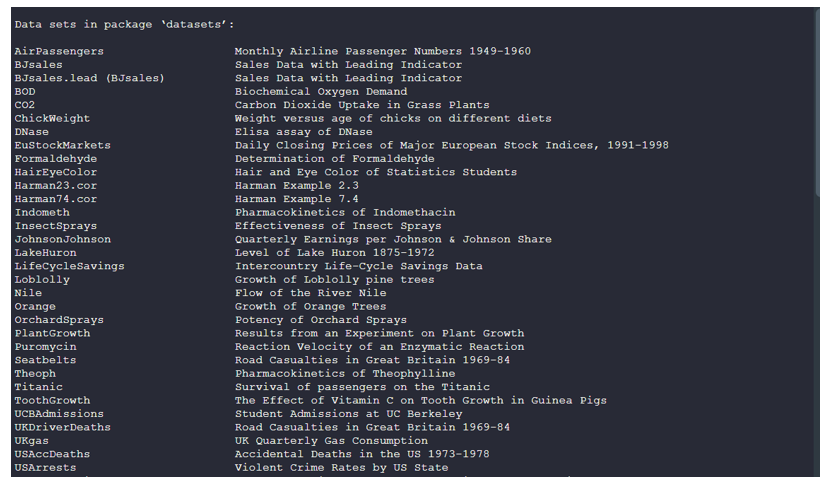
\includegraphics[width=0.5\textwidth]{3611_p7.png} % Directly insert image
\end{frame}  % <- Make sure this correctly ends the frame

\begin{frame}{Not Equal to Operator}
    \begin{itemize}
        \item \texttt{==} means equal to.
        \item \texttt{!=} means not equal to.
    \end{itemize}

    \textbf{Example:}
    
    \textbf{Keep only the rows where a certain value is 3:}
    \begin{itemize}
        \item dataFrame[value == 3,]
    \end{itemize}

    \textbf{Keep only the rows where a certain value is not 3:}
    \begin{itemize}
        \item dataFrame[value != 3,]
    \end{itemize}

\end{frame}


\begin{frame}[fragile]{\texttt{unique()} Function}
    \begin{itemize}
        \item Eliminate or delete the duplicate values:
    \end{itemize}

    \textbf{Example:}
    \begin{verbatim}
my_numbers <- c(1, 2, 2, 2, 4)
unique(my_numbers)

my_words <- c("pen", "university", "pen", "pen")
unique(my_words)
    \end{verbatim}
\end{frame}



\begin{frame}{\texttt{\%in\%} Operator}
    \begin{itemize}
        \item Check if elements of \texttt{vector1} are present in \texttt{vector2}:
    \end{itemize}

    \textbf{Example:}
    \begin{verbatim}
    
vector1 <- c(1, 2, 3, 4, 5)

vector2 <- c(3, 4, 5, 6, 7)
    \end{verbatim}
    \begin{itemize}
        \item \texttt{vector1 \%in\% vector2}
    \end{itemize}
\end{frame}  

\begin{frame}{Installed Packages in R}
    \textbf{The list of installed packages:}
    \begin{itemize}
        \item \texttt{my\_installed\_packages <- rownames(installed.packages())}
        \item \texttt{my\_installed\_packages}
    \end{itemize}
\end{frame}  

\begin{frame}{Popular R Packages}
    \textbf{Some mostly used and popular packages in R}
    \begin{itemize}
        \item To use a package in R:
        \begin{itemize}
            \item Install the package.
            \item Import its library.
        \end{itemize}
    \end{itemize}
    \centering
    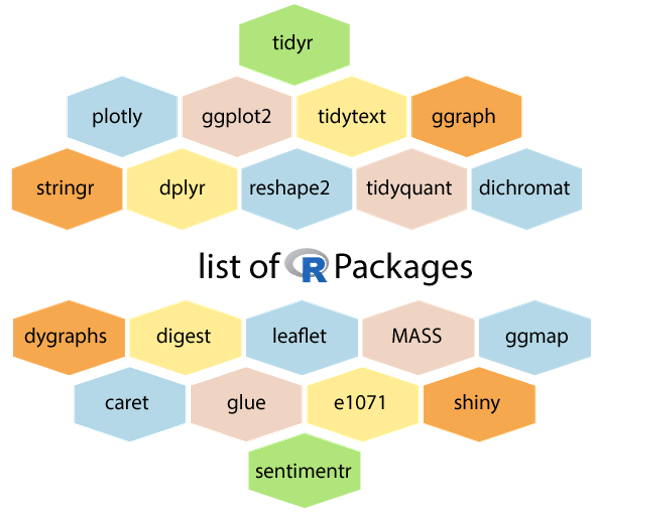
\includegraphics[width=0.5\textwidth]{3611_p8.png} % Corrected placement of image
\end{frame}  % <- Correctly closing this frame

\begin{frame}{Importing Libraries}
    \begin{itemize}
        \item Some functions are not available in R by default.
        \item You need to load the library before using its functions:
        \begin{itemize}
            \item \texttt{library(libraryName)}
        \end{itemize}
        \item Best practice: Load all required libraries at the beginning of your script.
    \end{itemize}
\end{frame}

\begin{frame}{\texttt{str\_detect} Function}
    \begin{itemize}
        \item Install the \texttt{stringr} package:
        \begin{itemize}
            \item \texttt{install.packages("stringr")}
        \end{itemize}
        \item Load the package:
        \begin{itemize}
            \item \texttt{library(stringr)}
        \end{itemize}
    \end{itemize}
\end{frame}

\begin{frame}{\texttt{str\_detect} Function}
    \begin{itemize}
        
        \item The \texttt{str\_detect()} function is used to detect patterns in strings.
        \item \texttt{unique()} extracts unique values from a column.
        \item The detected values are stored in a new variable.
        \item \texttt{str\_detect()} returns \texttt{TRUE} if a pattern is found in a string, otherwise \texttt{FALSE}.
    \end{itemize}
\end{frame}

\begin{frame}{Examples of \texttt{str\_detect()}}
    \begin{itemize}
        \item Define a vector of fruit names:
        \begin{itemize}
            \item \texttt{fruit <- c("apple", "banana", "pear", "pineapple")}
        \end{itemize}
        \item Detect if the letter "a" is in each fruit name:
        \begin{itemize}
            \item \texttt{str\_detect(fruit, "a")}
        \end{itemize}
        \item Check if a word **starts with** "a":
        \begin{itemize}
            \item \texttt{str\_detect(fruit, "\string^a")}
        \end{itemize}
        \item Check if a word **ends with** "a":
        \begin{itemize}
            \item \texttt{str\_detect(fruit, "a\$")}
        \end{itemize}
        \item Detect if the letter "b" is in the fruit names:
        \begin{itemize}
            \item \texttt{str\_detect(fruit, "b")}
        \end{itemize}
        \item Check if the word contains any vowels:
        \begin{itemize}
            \item \texttt{str\_detect(fruit, "[aeiou]")}
        \end{itemize}
    \end{itemize}
\end{frame}

\begin{frame}{\texttt{str\_detect()} Function with PlantGrowth Data}
    \begin{itemize}
        \item The \texttt{PlantGrowth} dataset is used in this example.
        \item \texttt{unique()} extracts unique values from a column.
        \item \texttt{str\_detect()} identifies values containing "trt".
        \item The detected values are stored in a new variable.
    \end{itemize}

    
    \begin{block}{Example Code:}
     \quad data(PlantGrowth)\\
\quad unique\_PlantGrowth = unique(PlantGrowth\$group)\\
\quad str\_detect(unique\_PlantGrowth, "trt1")\\
\quad my\_trt = unique\_PlantGrowth[str\_detect(unique\_PlantGrowth, "trt1")] 
    \end{block}


\end{frame}


\begin{frame}{For Loops in R}
    \begin{itemize}
        \item Best used when the number of iterations is known.
        \item A `for` loop executes a block of code multiple times.
        \item The loop variable takes values in the specified range.
    \end{itemize}
        \begin{block}{Function Syntax}
        \texttt{Loop\_functionName <- loop ( parameters ) \{\\
        \quad function Body Code\\
        \quad print( returnContents )\\
        \}}
    \end{block}
        \begin{block}{Example Function:A loop that prints numbers from `1` to `10`, adding `2` to each value.}
        \texttt{for\_loop <- for ( x in 1:10 ) \{\\
        \quad y <- x + 2\\
        \quad print( y )\\
        \}}
    \end{block}

\end{frame}
\begin{frame}{Correlation}
    \begin{itemize}
        \item \textbf{Inverse of a variable:} 
        \begin{itemize}
            \item The `1/variable` expression gives you the inverse, similar to other programming languages.
        \end{itemize}
        
        \item \textbf{Correlation:} 
        \begin{itemize}
            \item \texttt{cor(x, y)} gives the correlation value between variables \texttt{x} and \texttt{y}.
        \end{itemize}
    \end{itemize}
\end{frame}

\begin{frame}{Lab 4 - QQ Plots in R}
    \begin{itemize}
        \item \textbf{Quantile-Quantile Plot:} 
        \begin{itemize}
            \item \texttt{qqnorm(data)}
            \item Creates a quantile-quantile plot of the variables/data.
            \item Use \texttt{main=""} to set a title, like in histograms.
        \end{itemize}
        
        \item \textbf{QQ Line:} 
        \begin{itemize}
            \item \texttt{qqline(data)} draws a reference line in the QQ plot.
            \item Helps assess how well data fits a normal distribution.
            \item Customize with \texttt{qqline(data, col="blue", lwd=2)} to change color and line width.
        \end{itemize}
    \end{itemize}
\end{frame}

\begin{frame}{Lab Submissions}
    \begin{itemize}
        \item \textbf{R Script:}
        \begin{itemize}
            \item Must be well-commented.
            \item Should run without errors and match the report's output.
        \end{itemize}
        \item \textbf{Report:}
        \begin{itemize}
            \item Template available on Canvas.
            \item Add necessary explanations.
        \end{itemize}
        \item \textbf{Updated Note Sheet:} 
        \begin{itemize}
            \item For Lab 4: Include notes from Labs 1, 2, 3, and 4.
        \end{itemize}
    \end{itemize}
\end{frame}

\end{document}
